\documentclass[12pt]{article}
\usepackage[a4paper]{geometry}
\usepackage[pdftex]{hyperref}
\usepackage[german]{babel}
\usepackage[utf8]{inputenc}
\usepackage{csquotes}
\usepackage{amssymb}
\usepackage{graphicx}
\usepackage{multicol}
\usepackage{amsmath}
\usepackage{enumitem}
\usepackage{tabularx}
\usepackage{vwcol}
\usepackage{fancyhdr}
\usepackage{indentfirst}
\usepackage{polynom}

\geometry{
  headheight=14px,
  left=2.54cm,
  right=2.54cm,
  bottom=2cm,
  top=2cm
}

% For horizontally centering text in Y column
\newcolumntype{Y}{>{\centering\arraybackslash}X}

\setlength{\parindent}{0cm}

\setlength{\marginparsep}{1 cm}
\setlength{\topmargin}{-0.6in}
\setlength{\textheight}{9.5in}
\pagestyle{fancy}

% German-style quotation marks %
\MakeOuterQuote{"}

% Typesetting differential operator %
\providecommand\d{}
\renewcommand{\d}[1]{\:\mathrm{d}{#1}} 

% For vertical centering text in X/Y column
\renewcommand\tabularxcolumn[1]{m{#1}}

\polyset{%
   style=C,
   delims={\big(}{\big)},
   div=:
}

\fancypagestyle{firstpage}{%
  \lhead{\bf Staatliche Studienakademie Dresden\\
Studienrichtung: Informationstechnologie}
  \rhead{\bf Datum: 06.06.2020}
}

\cfoot{\thepage\ of \pageref*{LastTask}}


\begin{document}

\thispagestyle{firstpage}

\begin{flushright}
Anzahl der Klausurblätter: \pageref*{LastTask}
\end{flushright}

Klausur im Lehrgebiet: Algebra/Analysis\\

Teilgebiet: Analysis \\

Modulcode: 3IM-MATHE-10 \\

Lehrender: Andre Wachsmuth \\

Semester: 1 \\

\begin{vwcol}[widths={0.4,0.4,0.2},sep=0cm, justify=flush,rule=0pt,indent=4em]
Name:\\
Vorname:\\
SG:
\end{vwcol}

\bigskip
\bigskip
\bigskip
Bearbeitungszeit: 40 min \\

Zugelassene Hilfsmittel: 1 handbeschriebenes A4-Blatt \\

\textbf{Es dürfen keine eigenen Zusatzblätter abgegeben werden.} \\

\textbf{Verwenden Sie auch die Blattrückseiten für Antworten! Markieren Sie deutlich, zu welcher Frage die auf Rückseiten gegebenen Antworten gehören.} \\

\textbf {Der Rechengang muss eindeutig und vollständig ersichtlich sein!} \\

Punkteverteilung:

\bigskip

\begin{tabularx}{\textwidth}{l|Y|Y|Y|Y|Y}
Aufgabe        & 1 & 2 & 3 & 4  & Summe \\ [1ex] \hline
Soll-Punktzahl & 7 & 7 & 9 & 8  &       \\ [3ex]
Ist-Punktzahl  &   &   &   &    &       \\ [3ex]
\end{tabularx}

\newpage
\section* {Aufgabe 1}

In der folgenden Skizze ist das Richtungsfeld einer DGL 1. Ordnung sowie eine partikuläre Lösung $p$ eingetragen.

\begin{center}
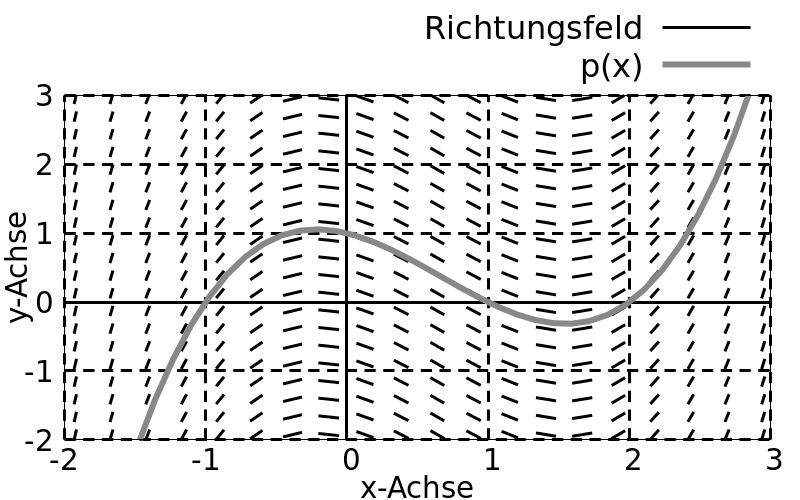
\includegraphics[width=0.95\textwidth]{grid.png}
\end{center}

\begin{enumerate}[label=(\alph*)]
\item (2P) Geben Sie ein Anfangswertproblem an, für das $p$ die Lösung ist!

\bigskip
\bigskip
\bigskip
\bigskip
\bigskip
\bigskip
\bigskip

\item (2P) Tragen Sie in die Skizze die Lösung des Anfangswertproblems $y(1) = -1$ ein!

\bigskip
\bigskip
\bigskip

\item (3P) Bei der Lösung $p$ handelt es sich um ein Polynom 3. Grads, dessen höchster Koeffizient $a_3=1/2$ beträgt. Finden Sie eine mögliche Funktionsgleichung für p! Hinweis: Fundamentalsatz der Algebra.

\bigskip
\bigskip
$p(x) = $

\end {enumerate}

\newpage
\section* {Aufgabe 2} Es werde der Pseudocode eines Computerprogramms betrachtet. Gesucht ist die Gesamtzeit $T$, die das Programm wartet.

\begin{verbatim}
Für n von 1 bis N:
  Für k von 1 bis n:
    Warte k Sekunden;
\end{verbatim}

Für die arithmetische und quadratische Reihe gelten folgende Formeln:

\begin{align*}
\sum\limits_{k=1}^n k   &= \frac{1}{2}n(n+1)\\
\sum\limits_{k=1}^n k^2 &= \frac{1}{6}n(n+1)(2n+1)
\end{align*}

\begin{enumerate}[label=(\alph*)]

\item (2P) Begründen Sie, dass die Gesamtwartezeit sich schreiben lässt als $T=\sum\limits_{n=1}^{N}\sum\limits_{k=1}^n k$

\bigskip
\bigskip
\bigskip
\bigskip
\bigskip
\bigskip
\bigskip

\item (5P) Berechnen Sie für $N=10$ die Gesamtwartezeit $T$ (in Sekunden)!

\bigskip
\bigskip
\bigskip
\bigskip
\bigskip
\bigskip
\bigskip
\bigskip
\bigskip
\bigskip
\bigskip
\bigskip
\bigskip
\bigskip
\bigskip
\bigskip
\bigskip
\bigskip
\bigskip
\bigskip
\bigskip

\textbf{Zusatzaufgabe (2P)} Welche (asymptotische) (Zeit-)Komplexität hat das Program bezogen auf $N$?

\end{enumerate}

\newpage
\section* {Aufgabe 3}

Gesucht ist ein Näherungswert für $\Gamma(2{,}8)$. Hierzu werde die Taylorentwicklung \textbf{2. Grads} der Gammafunktion $\Gamma(x)$ an der \textbf{Entwicklungsstelle} {$\mathbf{x_0=3}$ betrachtet. Folgende Werte der Gammafunktion benötigen Sie möglicherweise:


$$\Gamma(n) = (n-1)! \text{ für } n \in \mathbb{N}^{+}$$

\begin{center}
\begin{tabular}{ c | c | c | c | c}
 $\Gamma'(3)$ & $\Gamma''(3)$ & $\Gamma'''(3)$ & $\Gamma''''(3)$ & $\Gamma'''''(3)$ \\
 \hline
 1{,}85         &  2{,}50         & 3{,}45           &  5{,}52           & 8{,}85
\end{tabular}
\end{center}

\begin{enumerate}[label=(\alph*)]

\item (5P) Ermitteln Sie mit der Taylorentwicklung einen Näherungswert für $\Gamma(2{,}8)$ auf 2 Kommastellen genau!

Taylorformel: $\sum\limits_{k=0}^n\frac{\Gamma^{(k)}(x_0)}{k!}(x-x_0)^k$

\bigskip
\bigskip
\bigskip
\bigskip
\bigskip
\bigskip
\bigskip
\bigskip
\bigskip
\bigskip
\bigskip
\bigskip
\bigskip
\bigskip
\bigskip
\bigskip
\bigskip

\item (4P) Schätzen Sie den Fehler auf den in (a) ermittelten Wert ab (auf 3 Kommstellen genau)!\\
Hinweis: Für $x>2$ ist $\Gamma'''(x)$ streng monoton steigend.

Restgliedabschätzung: $|R_n(x)| \le \frac{|x_0-x|^{n+1}}{(n+1)!}\cdot\max\limits_{\vartheta\in[x_0,x]} |f^{(n+1)}(\vartheta)|$


\end{enumerate}

\newpage
\section* {Aufgabe 4}

Es werde die DGL $\frac{\cos(x^2)}{y'} = \frac{1}{2xy}$ betrachtet.

\begin{enumerate}[label=(\alph*)]

\item (3P) Erläutern Sie stichpunktartig die Struktur der Lösung einer linearen inhomogenen DGL n.-ter Ordnung mit konstanten Koeffzienten! Nutzen Sie dazu die Begriffe "Fundamentallösung", "Linearkombination", "homogene DGL", "inhomogene DGL" , "partikuläre Lösung" und "allgemeine Lösung"!

\bigskip
\bigskip
\bigskip
\bigskip
\bigskip
\bigskip
\bigskip
\bigskip
\bigskip
\bigskip
\bigskip
\bigskip
\bigskip
\bigskip
\bigskip
\bigskip

\item (5P) Finden Sie die allgemeine Lösung der DGL durch Trennung der Variablen. Das Integral über $x$ können Sie mit der Substitution $z=x^2$ lösen.


\end{enumerate}

\label{LastTask}

\newpage

\begin{center}
{\bf {\large Musterlösung}}
\end{center}

\begin{center}
{\bf {\large Klausur Analysis (3IT19, 3MI19) - 06.06.2020}}
\end{center}

\begin{center}
\textbf{Jeder Anführungspunkt entspricht einem erteilten Bewertungspunkt.} 

Ist ein Rechenschritt falsch, werden für darauf basierende Rechnungen Punkte erteilt (Folgefehler), es sei denn, die Rechnung wird dadurch wesentlich vereinfacht. 
\end{center}

\begin{enumerate}

% Task 1
\item
\begin{enumerate}

\item Etwa $y(1) = 0$ oder $y(0) = 1$	
\begin{itemize}
\item Für die mathematische korrekte Schreibweise eines Anfangswertproblems
\item Für ein mögliches Anfangswertproblem
\end{itemize}

\item Es muss eine Funktion zu $p$ um 1 nach unten verschobene Funktion eingetragen sein.
\begin{itemize}
\item Der Funktionsgraph verläuft durch $(1;-1)$
\item Der Funktionsgraph folgt etwa den eingezeichneten Richtungslinien
\end{itemize}

\item $p(x) = \frac{1}{2}(x+1)(x-1)(x-2)$
\begin{itemize}
\item Form ist korrekt (Produkt von Linearfaktoren mit Koeffizient)
\item Wert für Koeffizienten ist korrekt
\item Werte für Nullstellen sind korrekt
\end{itemize}

\end{enumerate}

% Task 2
\item
\begin{enumerate}

\item Jede schlüssige und grammatikalisch verständliche Begründung wird akzeptiert.
\begin{itemize}
\item Hintereinanderausführung der Aktion "Warten" resultiert in einer Wartezeit, welche die Summe beider Wartezeiten ist, daher kann die Summenschreibweise $\sum$ genutzt werden.
\item In der ersten Schleife wird von 1 bis $N$ iteriert, in inneren Schleife von 1 bis zur Zählvariable der ersten Schleife.
\end{itemize}

\item
\begin{itemize}
\item $T=\sum\limits_{n=1}^{10}\sum\limits_{k=1}^n k$
\item $=\sum\limits_{n=1}^{10} \frac{1}{2}(n^2+n)$
\item $=\frac{1}{2} \cdot (\underbrace{\sum\limits_{n=1}^{10} n^2}_{ = \frac{1}{6}\cdot 10 \cdot 11 \cdot 21 = 5 \cdot 11 \cdot 7} + \underbrace{\sum\limits_{n=1}^{10} n}_{= 5\cdot 11})$
\item $ = \frac{1}{2}(55+385)$
\item $= 220$
\end{itemize}

\end{enumerate}

\bigskip

\textbf{Zusatzaufgabe}: $\mathbb{O}(N^3)$ bzw. $\Theta(N^3)$. 1P auf Notation, 1P auf Richtigkeit.

\newpage

% Task 3

\item
\begin{enumerate}

\item
\begin{itemize}
\item $\Gamma(x) \approx 2 + \Gamma'(3)(x-3) + \frac{\Gamma''(3)}{2!}(x-3)^2$
\item $\Gamma(x) \approx 2 + 1{,}85(x-3) + 1{,}25(x-3)^2$
\item $\Gamma(2{,}8) \approx 2{,}00 - 1{,}85 / 5 + 1{,}25\cdot {0.04}$
\item $= 2{,}00 - 0{,}37 + 0{,}05$
\item $= 1{,}68$
\end{itemize}

\item
\begin{itemize}
\item $|R_2(2{,}8)| \le \frac{0{,}2^3}{6}\cdot\max\limits_{\vartheta \in [2{,}8;3{,}0]} |\Gamma'''(x)|$
\item Da $\Gamma'''$ monoton steigend, ist Maximalwert $\Gamma'''(3)= 3{,}45$ \\
      $|R_2(2{,}8)| \le \frac{0{,}2^3}{6}\cdot 3{,}45$
\item $ = 0{,}008\cdot 0{,}575$
\item $ = 0{,}0046 \approx 0{,}005$
\end{itemize}

\end{enumerate}

% Task 4

\item 
\begin{enumerate}

\item 
\begin{itemize}
\item Allgemeine Lsg. d. homog. DGL ist beliebige Linearkomb. d. Fundamentallsg.
\item Allgemeine Lsg. d. inhomog. DGL ist Lsg. der homog. DGL
\item Plus irgendeine partik. Lsg. der inhomog. DGL
\end{itemize}

\item 
\begin{itemize}
\item $\frac{\d{y}}{y} = 2x\cos(x^2)\d{x}$
\item $\int\frac{\d{y}}{y} = \int 2x\cos(x^2)\d{x}$
\item $\ln(|y|) = \int 2x\cos(z)\frac{\d{z}}{2x}$
\item $\ln(|y|) = \sin(x^2) + C$
\item $y = C \cdot e^{\sin(x^2)}$
\end{itemize}

\end{enumerate}

\end{enumerate}


\end{document}
